
\section{Proof of Concept: Replicator and Imitation Dynamics} \label{Lottery_Me}
\subsection{Outline}
The paper chosen to replicate imitation and replicator dynamics was \cite{RN30}, which models a two-stage lottery game. Refer to \ref{Lottery} for a description of the game and the strategy space $C$. \\

The paper implemented agent--based replicator $(\alpha = 1)$ and imitation $(\alpha = 0)$ dynamics. After each round, every agent $i$ randomly chooses another agent $j$ from the population, and calculates $q_i$, \\

\begin{align} \label{rep}
q_i = \Bigg[ \frac{|\pi_j - \pi_i|}{\Delta} \Bigg]^\alpha \mathbbm{1}_{\{\pi_j>\pi_i\}}, \quad  0 \leq \alpha \leq 1.\end{align} 

In the formulation, $\Delta$ scales the difference so that $0 \leq q_i \leq 1$, and $\Delta = 16$ in this two-stage lottery game. Each agent then changes from strategy $i$ to strategy $j$ if $q_i \geq r_i,$ $r_i \sim \mathsf{U}(0,1)$. \\

\subsection{Results Comparison}
The simulated results were compared to the paper for $\alpha = 0, 1, 0.5$, and are shown below. \\

\FloatBarrier 
\begin{figure}[!h]
  \begin{subfigure}[b]{0.45\textwidth}
    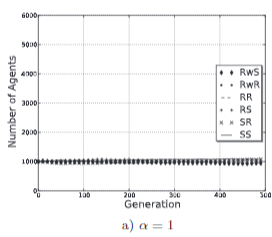
\includegraphics[width=\textwidth]{images/lottery1.png}
    \caption{Figure 5a from \cite{RN30}. The strategies SS, RR, SR, RS, R--WR, R--WS are represented by a solid line, crosses, plusses, dashes, dots and diamonds respectively. }
    \label{lottery1}
  \end{subfigure}
  \hfill
  \begin{subfigure}[b]{0.45\textwidth}
    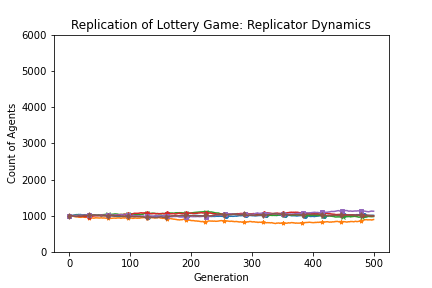
\includegraphics[width=1.25\textwidth]{images/lottery1_me.png}
    \caption{Replication of \ref{lottery1}. The strategies SS, RR, SR, RS, R--WR, R--WS are represented by blue circles, orange stars, green crosses, red pentagons, brown diamonds, and purple squares respectively.}
    \label{lottery1_me}
  \end{subfigure}
  \caption{Replication of Figure 5a from \cite{RN30}. The replication is successful, but these conditions do not provide anything interesting regarding replicator dynamics.} \label{lottery_comp0}
\end{figure} 
\FloatBarrier

\FloatBarrier 
\begin{figure}[!h]
  \begin{subfigure}[b]{0.45\textwidth}
    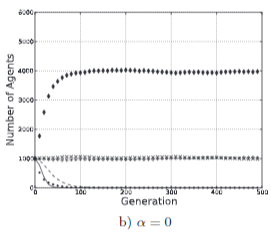
\includegraphics[width=\textwidth]{images/lottery2.png}
    \caption{Figure 5b from \cite{RN30}. The strategies SS, RR, SR, RS, R--WR, R--WS are represented by a solid line, crosses, plusses, dashes, dots and diamonds respectively. }
    \label{lottery2}
  \end{subfigure}
  \hfill
  \begin{subfigure}[b]{0.45\textwidth}
    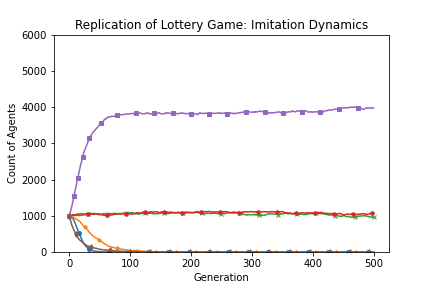
\includegraphics[width=1.25\textwidth]{images/lottery2_me.png}
    \caption{Replication of \ref{lottery2}. The strategies SS, RR, SR, RS, R--WR, R--WS are represented by blue circles, orange stars, green crosses, red pentagons, brown diamonds, and purple squares respectively.}
    \label{lottery2_me}
  \end{subfigure}
  \caption{Replication of Figure 5b from \cite{RN30}. The results are well replicated, and this model for imitation dynamics can be explored on other games.} \label{lottery_comp1}
\end{figure} 
\FloatBarrier



\FloatBarrier 
\begin{figure}[!h]
  \begin{subfigure}[b]{0.45\textwidth}
    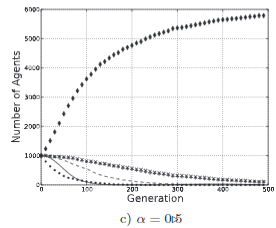
\includegraphics[width=\textwidth]{images/lottery3.png}
    \caption{Figure 5c from \cite{RN30}. The strategies SS, RR, SR, RS, R--WR, R--WS are represented by a solid line, crosses, plusses, dashes, dots and diamonds respectively. }
    \label{lottery3}
  \end{subfigure}
  \hfill
  \begin{subfigure}[b]{0.45\textwidth}
    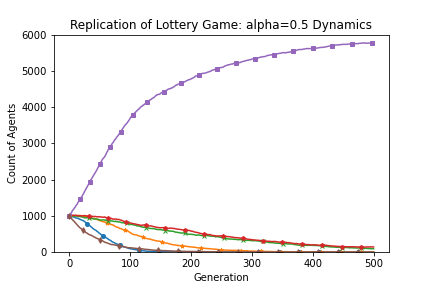
\includegraphics[width=1.25\textwidth]{images/lottery3_me.png}
    \caption{Replication of \ref{lottery3}. The strategies SS, RR, SR, RS, R--WR, R--WS are represented by blue circles, orange stars, green crosses, red pentagons, brown diamonds, and purple squares respectively. }
    \label{lottery3_me}
  \end{subfigure}
  \caption{Replication of Figure 5c from \cite{RN30}. This is neither true imitation or replicator dynamic, but provides an intermediary case.} \label{lottery_comp2}
\end{figure} 
\FloatBarrier


 It is also interesting to examine the results when the lottery win probability $p$ is not 0.5. For replicator dynamics, the strategy with the highest expected value eventually wins out, but for imitation dynamics the result is not so obvious. This was shown in Figure 6 from \cite{RN30}, and replicated below. For $p=0.4$, the expectation--maximising strategy is SS, but R--WS has an evolutionary advantage and takes over the population. This is supported by theoretical results in \cite{RN30}. Similarly, for $p=0.55$, the expectation--maximising strategy is RR, but R--WS also takes over the population. \\
 
 \FloatBarrier 
\begin{figure}[!h]
  \begin{subfigure}[b]{0.45\textwidth}
    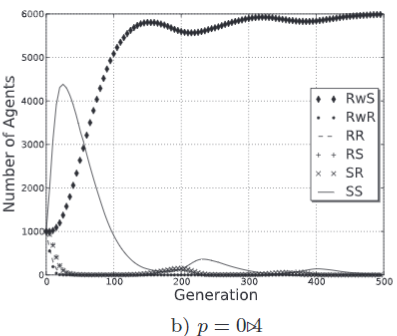
\includegraphics[width=\textwidth]{images/lotteryp4.png}
    \caption{Figure 6b from \cite{RN30}. The strategies SS, RR, SR, RS, R--WR, R--WS are represented by a solid line, crosses, plusses, dashes, dots and diamonds respectively.}
    \label{lotteryp4}
  \end{subfigure}
  \hfill
  \begin{subfigure}[b]{0.45\textwidth}
    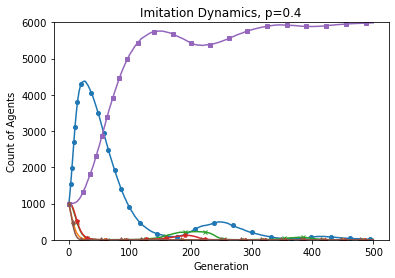
\includegraphics[width=1.25\textwidth]{images/lotteryp4_me.png}
    \caption{Replication of \ref{lotteryp4}. The strategies SS, RR, SR, RS, R--WR, R--WS are represented by blue circles, orange stars, green crosses, red pentagons, brown diamonds, and purple squares respectively. }
    \label{lotteryp4_me}
  \end{subfigure}
  \caption{Replication of Figure 6b from \cite{RN30}. Although SS is the expectation--maximising strategy, it is not an ESS, and R--WS has the evolutionary advantage.} \label{lottery_comp4}
\end{figure} 
\FloatBarrier

 \FloatBarrier 
\begin{figure}[!h]
  \begin{subfigure}[b]{0.45\textwidth}
    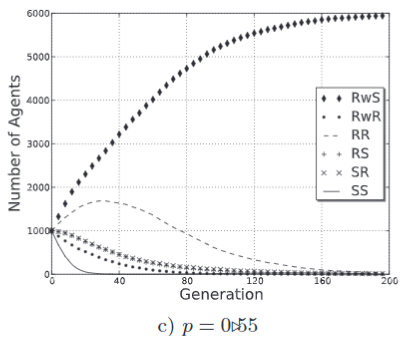
\includegraphics[width=\textwidth]{images/lotteryp055.png}
    \caption{Figure 6c from \cite{RN30}. The strategies SS, RR, SR, RS, R--WR, R--WS are represented by a solid line, crosses, plusses, dashes, dots and diamonds respectively.}
    \label{lotteryp055}
  \end{subfigure}
  \hfill
  \begin{subfigure}[b]{0.45\textwidth}
    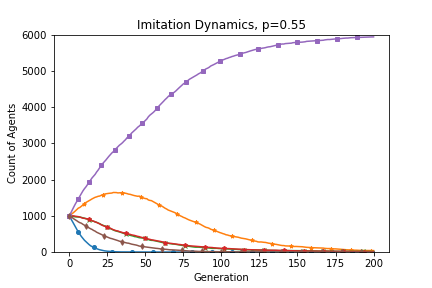
\includegraphics[width=1.25\textwidth]{images/lotteryp055_me.png}
    \caption{Replication of \ref{lotteryp055}. The strategies SS, RR, SR, RS, R--WR, R--WS are represented by blue circles, orange stars, green crosses, red pentagons, brown diamonds, and purple squares respectively. }
    \label{lotteryp4_me_2}
  \end{subfigure}
  \caption{Replication of Figure 6c from \cite{RN30}. In this case, RR is expectation--maximising, but R--WS still wins out.} \label{lottery_comp5}
\end{figure} 
\FloatBarrier

\subsection{Extension}
In \cite{RN30}, plots for $p=0.3, 0.7$ were also shown, however the expectation--maximising strategies win out quickly, so they are not included here. It is notable that in Figure \ref{lotteryp4_me}, there are some fluctuations that occur before stability. Consider the three strategies RS, SS, R--WS under the $p=0.4$ regime. The strategy RS is the same as SR, because the order of the lottery does not matter. Their distributions are shown below. \\
\begin{align*}
    \mathbb P_{\text{RS}}(x = \pi)  &= \begin{cases} 0.4 \quad \pi = 12 \\
    0.6 \quad \pi =4 
    \end{cases}, \\
        \mathbb P_{\text{R--WS}}(x = \pi)  &= \begin{cases} 0.4 \quad \pi = 12 \\
    0.24 \quad \pi =8 \\
    0.36 \quad \pi = 0\\
    \end{cases}, \\
    \mathbb P_{\text{SS}}(x = \pi)  &= \mathbbm{1}_{\pi = 8}.
\end{align*}
Under imitation dynamics, a strategy $i$ has an evolutionary advantage over $j$, $j \prec i$, if $\mathbb P(\pi_i > \pi_j) > \mathbb P(\pi_i < \pi_j)$. In the example above, RS $\prec$ SS $\prec$ R--WS $\prec$ RS, which is a cycle. In \ref{lotteryp4_me}, the strategy SS eliminates RS much faster than RS can eliminate R--WS, so SS temporarily grows, and then succumbs to R--WS. Under imitation dynamics, once a strategy is eliminated it can never return, and the elimination of RS ensures the eventual dominance of R--WS. The image in \ref{lotteryp4_me} is aggregated over 20 trials, and the time to elimination is quite variable. The empirical quantiles are shown below, instead computed over 120 trials.  \\

\FloatBarrier
\graphCap{lotteryp4_me_quantiles_empirical.png}{0.75}{Empirical 2.5\%, 97.5\% Quantiles of Imitation Dynamics Lottery Game, $p=0.4$, T = 120. The strategies SS, RR, SR, RS, R--WR, R--WS are represented by blue circles, orange stars, green crosses, red pentagons, brown diamonds, and purple squares respectively. The quantile for each series is the dashed line. }{lottery_quantiles_empirical}
\FloatBarrier
Figure \ref{lottery_quantiles_empirical} shows how great the variance of certain series are, particularly SS and R--WS. When R--WS is prominent and the strategies SR, RS are not extinct, SR, RS are able to grow. This occurs around the 200th generation. The strategy SS, which outperforms SR and RS, then dominates them. SS is dominated by R--WS, and this cycle continues until SR and RS are eliminated. The reason that they are eliminated is because the highest rate of dominance is SS over SR, RS. \\
\FloatBarrier
\graphCap{lotteryp4_me_quantiles.png}{0.75}{95\% Confidence Interval for the Mean, Imitation Dynamics Lottery Game, $p=0.4$, T = 120. The strategies SS, RR, SR, RS, R--WR, R--WS are represented by blue circles, orange stars, green crosses, red pentagons, brown diamonds, and purple squares respectively. The confidence interval for each series is the dashed line. }{lottery_quantiles}
\FloatBarrier
 The computed confidence intervals assume a normal distribution of the mean under the Central Limit Theorem. The computed standard deviation of each point in the time series is used as an estimate of the true standard deviation. Because the number of trials $T=120$, the confidence interval is tight around the sample mean. The original paper uses $T=20$, which results in a confidence interval four times as wide Figure \ref{lottery_quantiles}. Therefore it is suggested that more than 20 trials are used for future samples. \\



\subsection{Summary}
The purpose of replicating \cite{RN30} was to demonstrate replicator and imitation dynamics. This demonstration was achieved, and now these dynamics can be applied to the PGG. A cycle of strategies was demonstrated for imitation dynamics under a $p=0.4$ regime. Although the original paper did not investigate the distribution of results, they are discussed above. The paper \cite{RN30} did not use an underlying network structure, but the dynamics can easily be transposed onto a graph by limiting the sample space of agents to neighbours. \\


\section{Local Replicator Dynamics for Public Good Games}
\subsection{Outline}
The following section investigates the effect of graph model on cooperation under local replicator dynamics. The graph models from \ref{other_networks} are also investigated here, and sample characteristics are given in Table \ref{graph_stats}. The game is played by a population of 500 agents, where each agents hosts a play of the PGG with their neighbours. After every agent has hosted, the agent--based replicator dynamics from \eqref{rep} are implemented on each agent's neighbourhood. Each plot aggregates the mean of each series over 80 trials.  \\
\subsection{Results}
\graphCap{replicator_graphs_low}{0.8}{Comparing Graph Models: Replicator Dynamics. Trend for $r \in \{2, 2.5, 3, 3.5\}$. In each graph, the blue circles, orange stars, green crosses, and red pentagons correspond to the WS model, TAG model, BA model, and RRG model respectively. }{replicator_low} 

\graphCap{replicator_graphs_medium}{0.8}{Comparing Graph Models: Replicator Dynamics. Trend for $r \in \{4,4.5,5,5.5\}$. In each graph, the blue circles, orange stars, green crosses, and red pentagons correspond to the WS model, TAG model, BA model, and RRG model respectively. }{replicator_medium}

\graphCap{replicator_graphs_large}{0.8}{Comparing Graph Models: Replicator Dynamics. Trend for $r \in \{6,6.5,7,7.5\}$. In each graph, the blue circles, orange stars, green crosses, and red pentagons correspond to the WS model, TAG model, BA model, and RRG model respectively. }{replicator_large}

Replicator dynamics result in slower convergence than the satisfaction model in Chapter \ref{TA}. Therefore the number of generations has been extended to 200, so that equilibrium is observed. Figure \ref{replicator_low} shows the TAG and BA model inducing higher cooperation than WS, RRG models. This trend continues for $2.5 \leq r \leq 7.5$. It appears that graph models with a power law degree size distribution induce higher cooperation. In Chapter \ref{C1} it is hypothesised that the presence of high--degree nodes is sufficient to induce cooperation across the network, which corroborrates the trend observed here. \\

\subsection{Controlling for Degree Size Distribution}
To test the hypothesis that the average clustering coefficient $C_\Delta$ does not impact cooperation, the \verb+power_law+ package was used to create another graph model, denoted PL. It induces a degree distribution with power law shape, but the parameter $p$ dictates the clustering coefficient. After each node is connected, the parameter $p$ determines the probability that the next link joins two neighbours, completing the triangle. Two degree histograms are plotted below, which emphasise the degree size distribution. \\
\graphCap{PL01BA.png}{0.5}{Comparison of Power Law Clustering Graph with BA model, $p=0.1$. The degree histograms are similar, so the only difference is the clustering coefficient.}{PL01BA}

\graphCap{PL05BA.png}{0.5}{Comparison of Power Law Clustering Graph with BA model, $p=0.5$. The degree histograms are similar, so the only difference is the clustering  coefficient.}{PL05BA}

\begin{table}[!h]
\begin{center}
\begin{tabular}{|l|l|l|l|l|}
\hline
Graph Type & Mean Degree & $l$ & $C_\Delta$ & Degree Variance \\ \hline
PL: $p=0.1$        & 5.96        & 3.234                         & 0.10                   & 42.35           \\ \hline
PL: $p=0.2$        & 5.96           & 3.24                         & 0.15                   & 44.07               \\ \hline
PL: $p=0.4$       & 5.96        & 3.25                         & 0.25                   & 47.92           \\ \hline
PL: $p=0.6$         & 5.96           & 3.30                         & 0.35                   & 49.92            \\ \hline
\end{tabular}
\caption{Computed characteristics for PL graph, varying cluster parameter $p$. The characteristics were computed over 100 samples of each graph, and then averaged. } \label{graph_stats}
\end{center}
\end{table}

\graphCap{comparing_power_p_low.png}{0.5}{In each graph, the blue circles, orange stars, green crosses, red pentagons, and purple squares correspond to $p=[0.1,0.2,0.3,0.4,0.5]$ respectively.}{power_p_low}

\graphCap{comparing_power_p_high.png}{0.5}{In each graph, the blue circles, orange stars, green crosses, red pentagons, and purple squares correspond to $p=[0.1,0.2,0.3,0.4,0.5]$ respectively.}{power_p_high}


